
% LaTeX code to include the three distractor latch figures as subplots

\begin{figure}[htbp]
    \centering
    \begin{subfigure}[b]{0.48\textwidth}
        \centering
        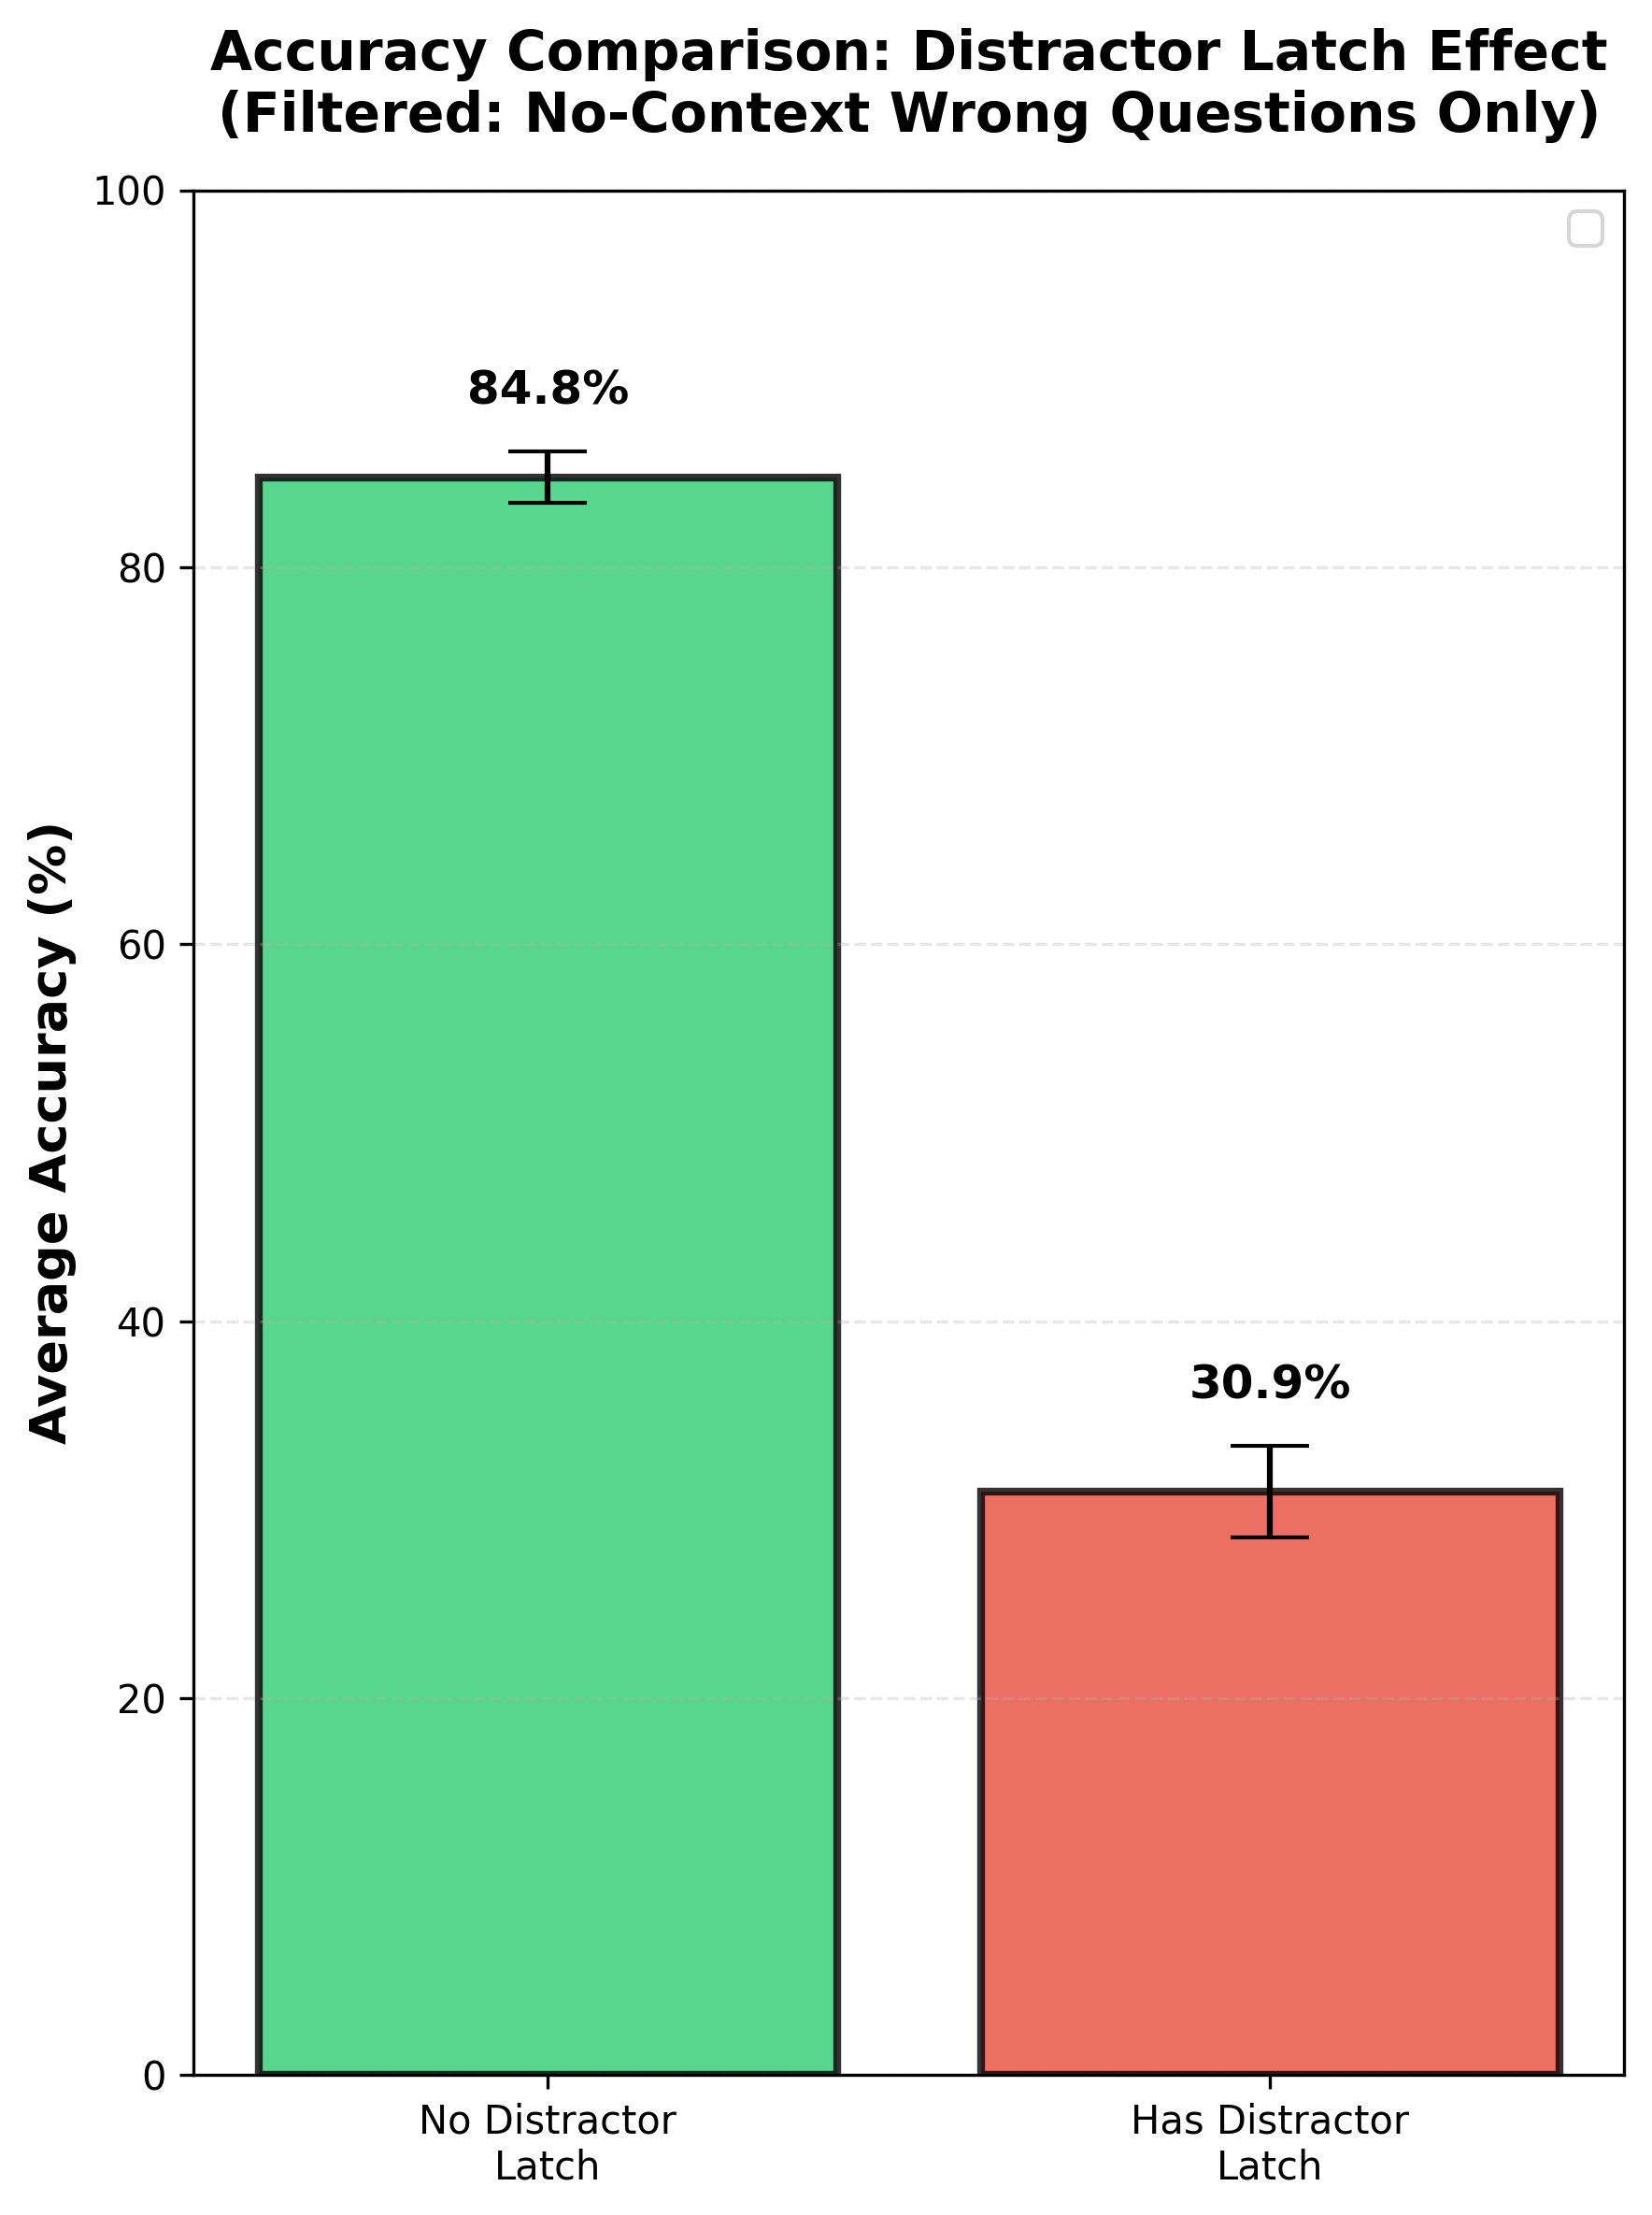
\includegraphics[width=\textwidth]{distractor_latch_accuracy_comparison.png}
        \caption{Overall accuracy comparison showing the impact of distractor latch on model performance.}
        \label{fig:distractor_accuracy}
    \end{subfigure}
    \hfill
    \begin{subfigure}[b]{0.48\textwidth}
        \centering
        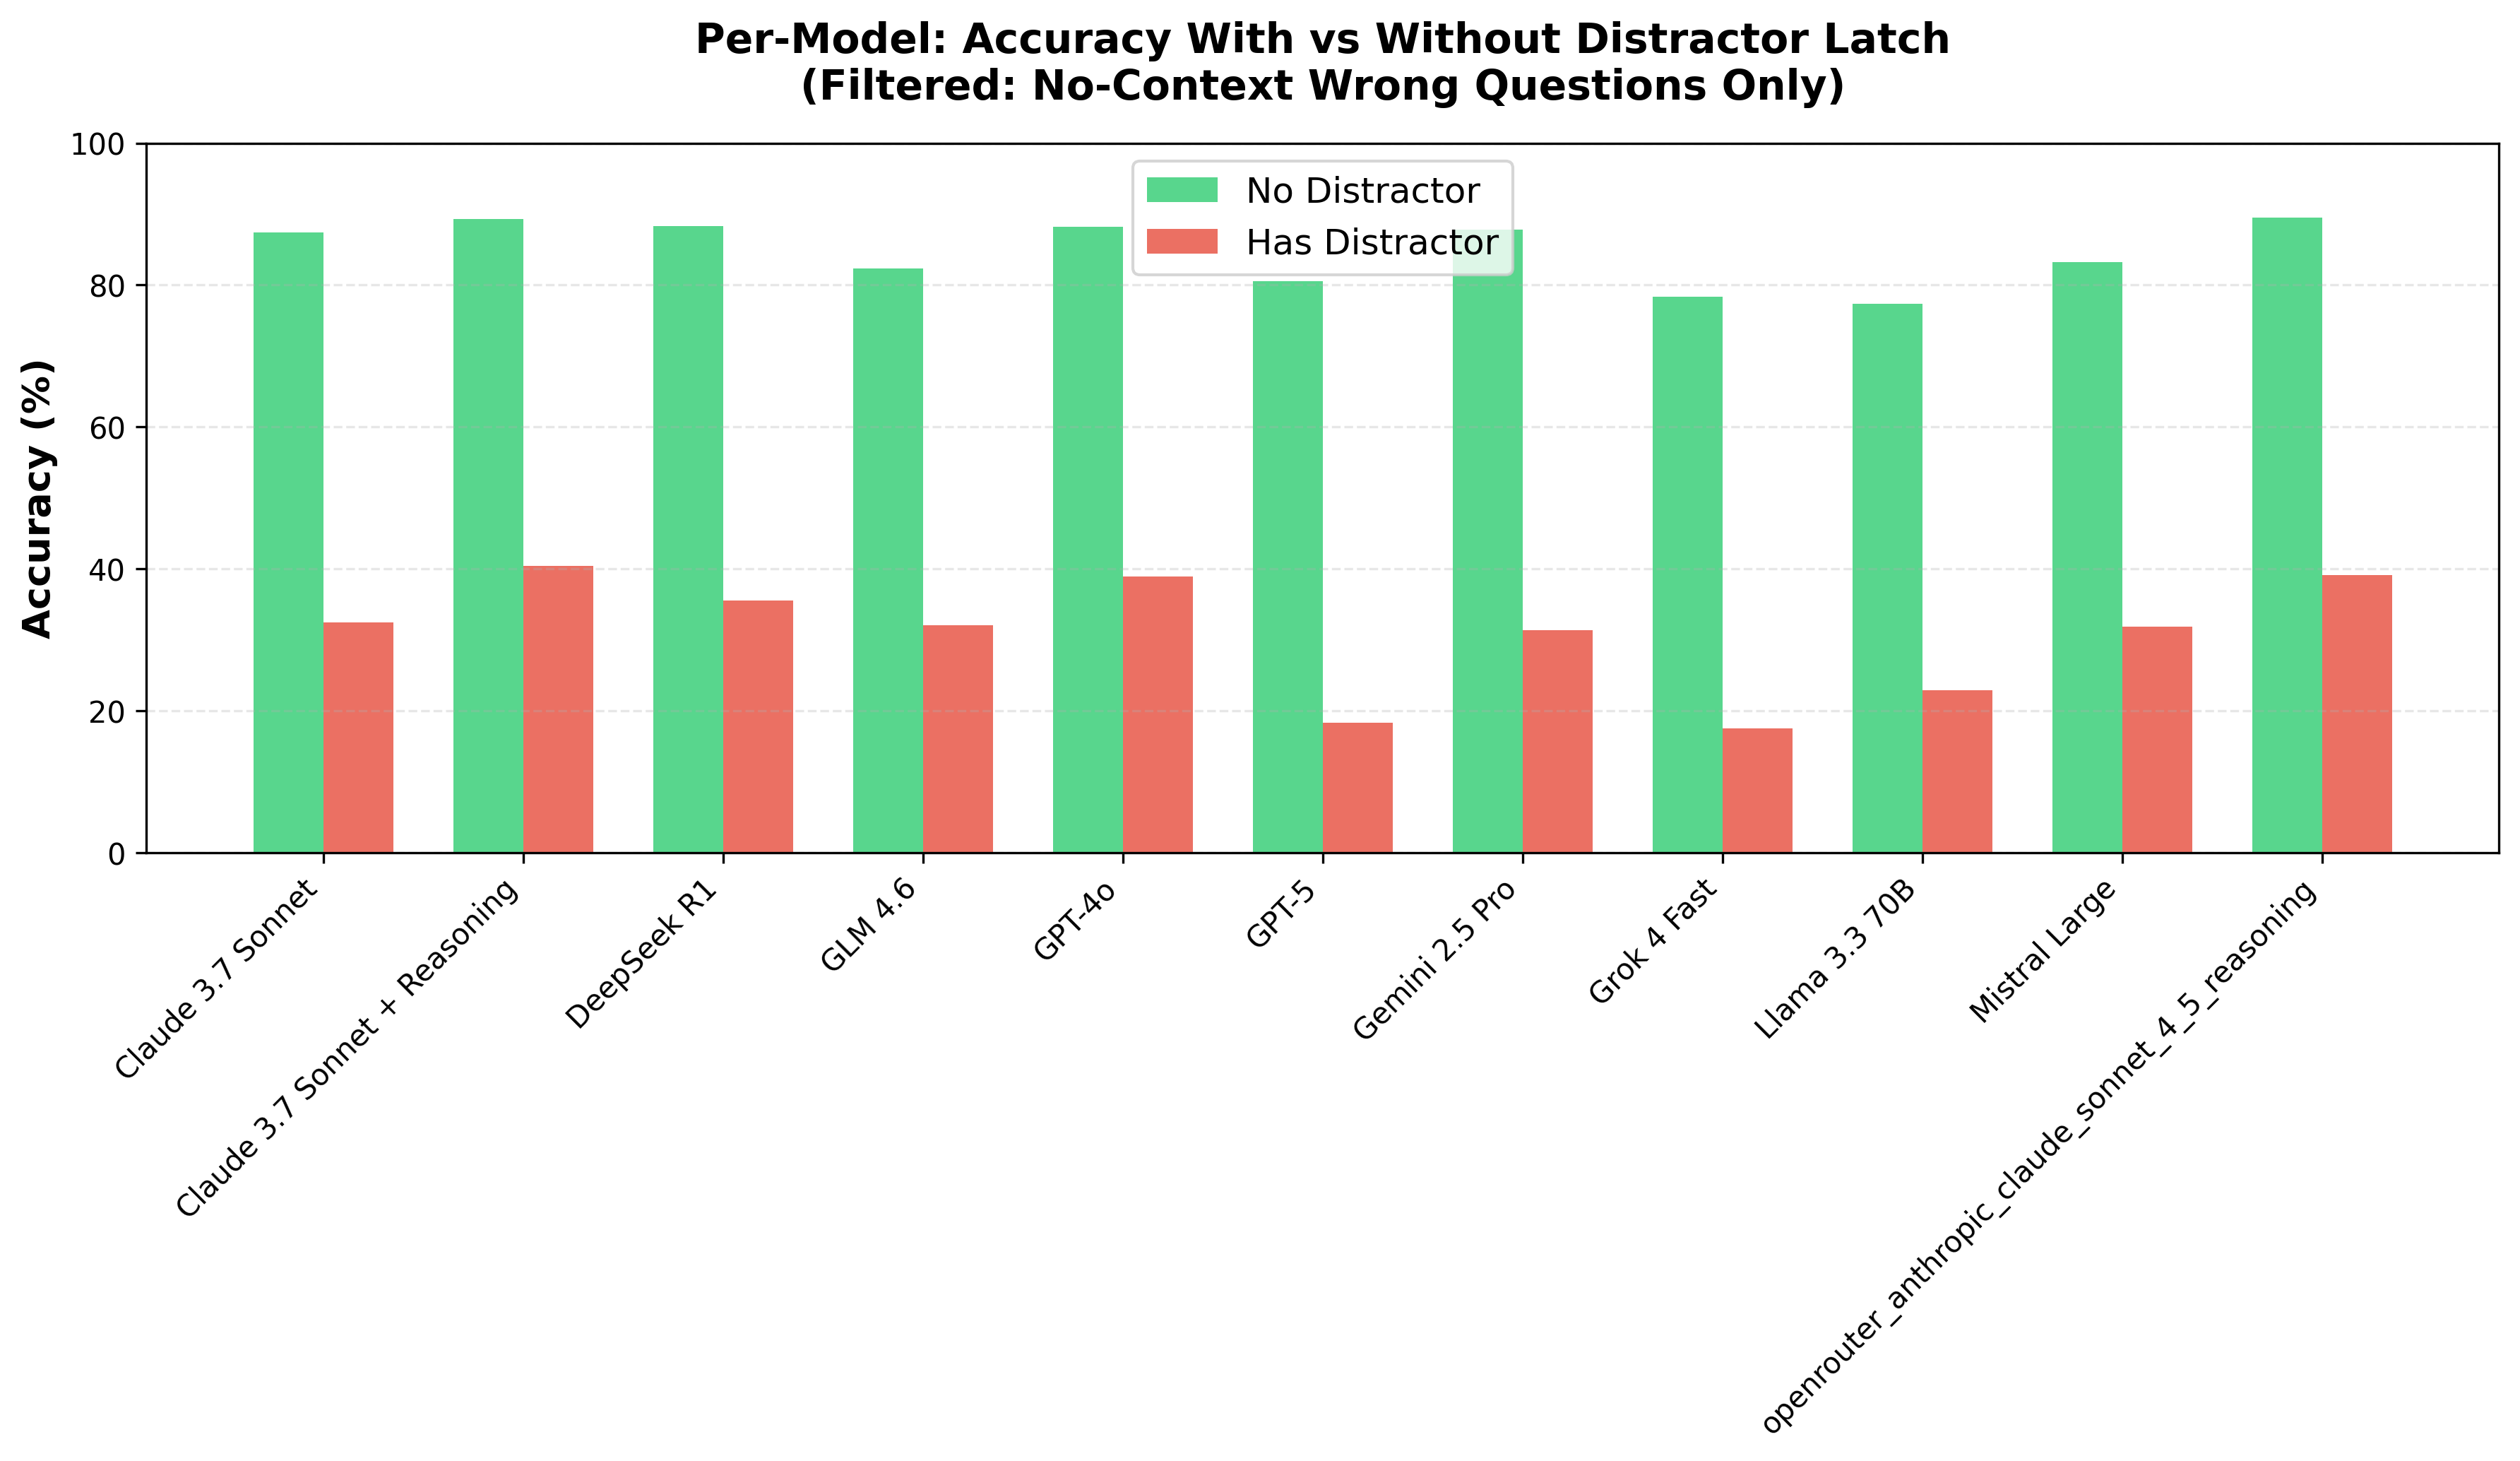
\includegraphics[width=\textwidth]{distractor_latch_per_model.png}
        \caption{Per-model accuracy breakdown comparing questions with and without distractor latch.}
        \label{fig:distractor_per_model}
    \end{subfigure}
    
    \vspace{0.5cm}
    
    \begin{subfigure}[b]{0.65\textwidth}
        \centering
        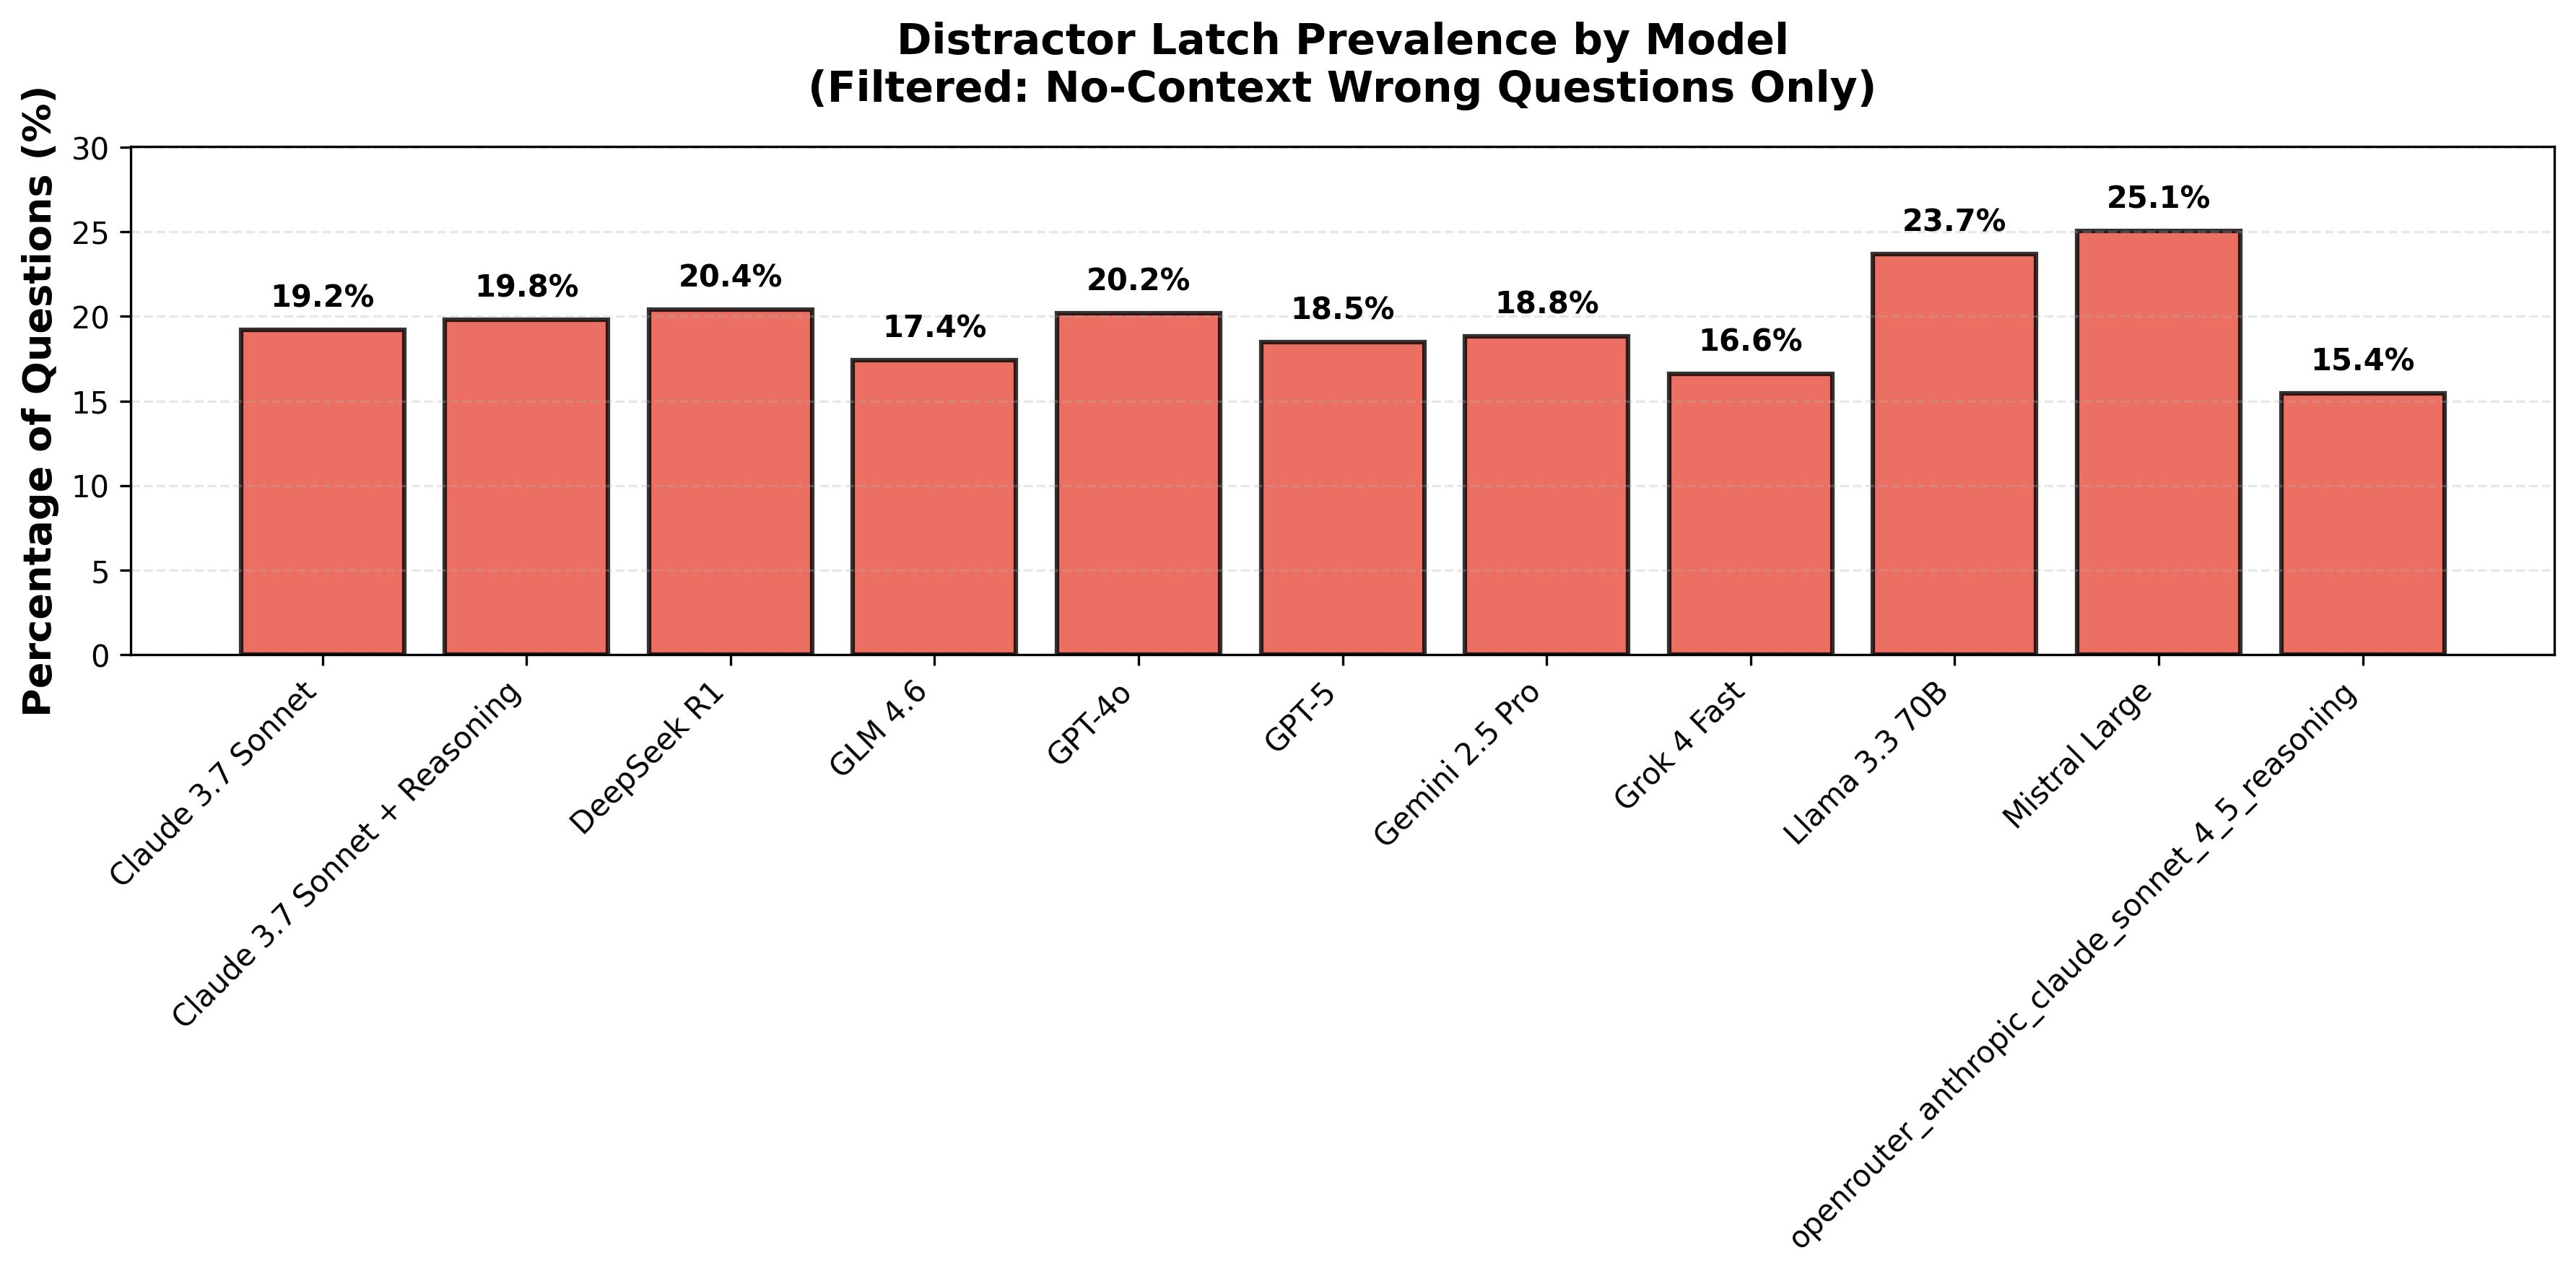
\includegraphics[width=\textwidth]{distractor_latch_prevalence.png}
        \caption{Prevalence of distractor latch across different models.}
        \label{fig:distractor_prevalence}
    \end{subfigure}
    
    \caption{Analysis of distractor latch effects on iterative RAG performance. (a) shows the overall accuracy drop of 52 percentage points when distractor latch occurs, (b) demonstrates this effect consistently across all models, and (c) reveals varying prevalence rates by model.}
    \label{fig:distractor_latch_analysis}
\end{figure}

% Alternative: Horizontal layout (all three in one row)
% Uncomment below if you prefer a single-row layout:

% \begin{figure}[htbp]
%     \centering
%     \begin{subfigure}[b]{0.32\textwidth}
%         \centering
%         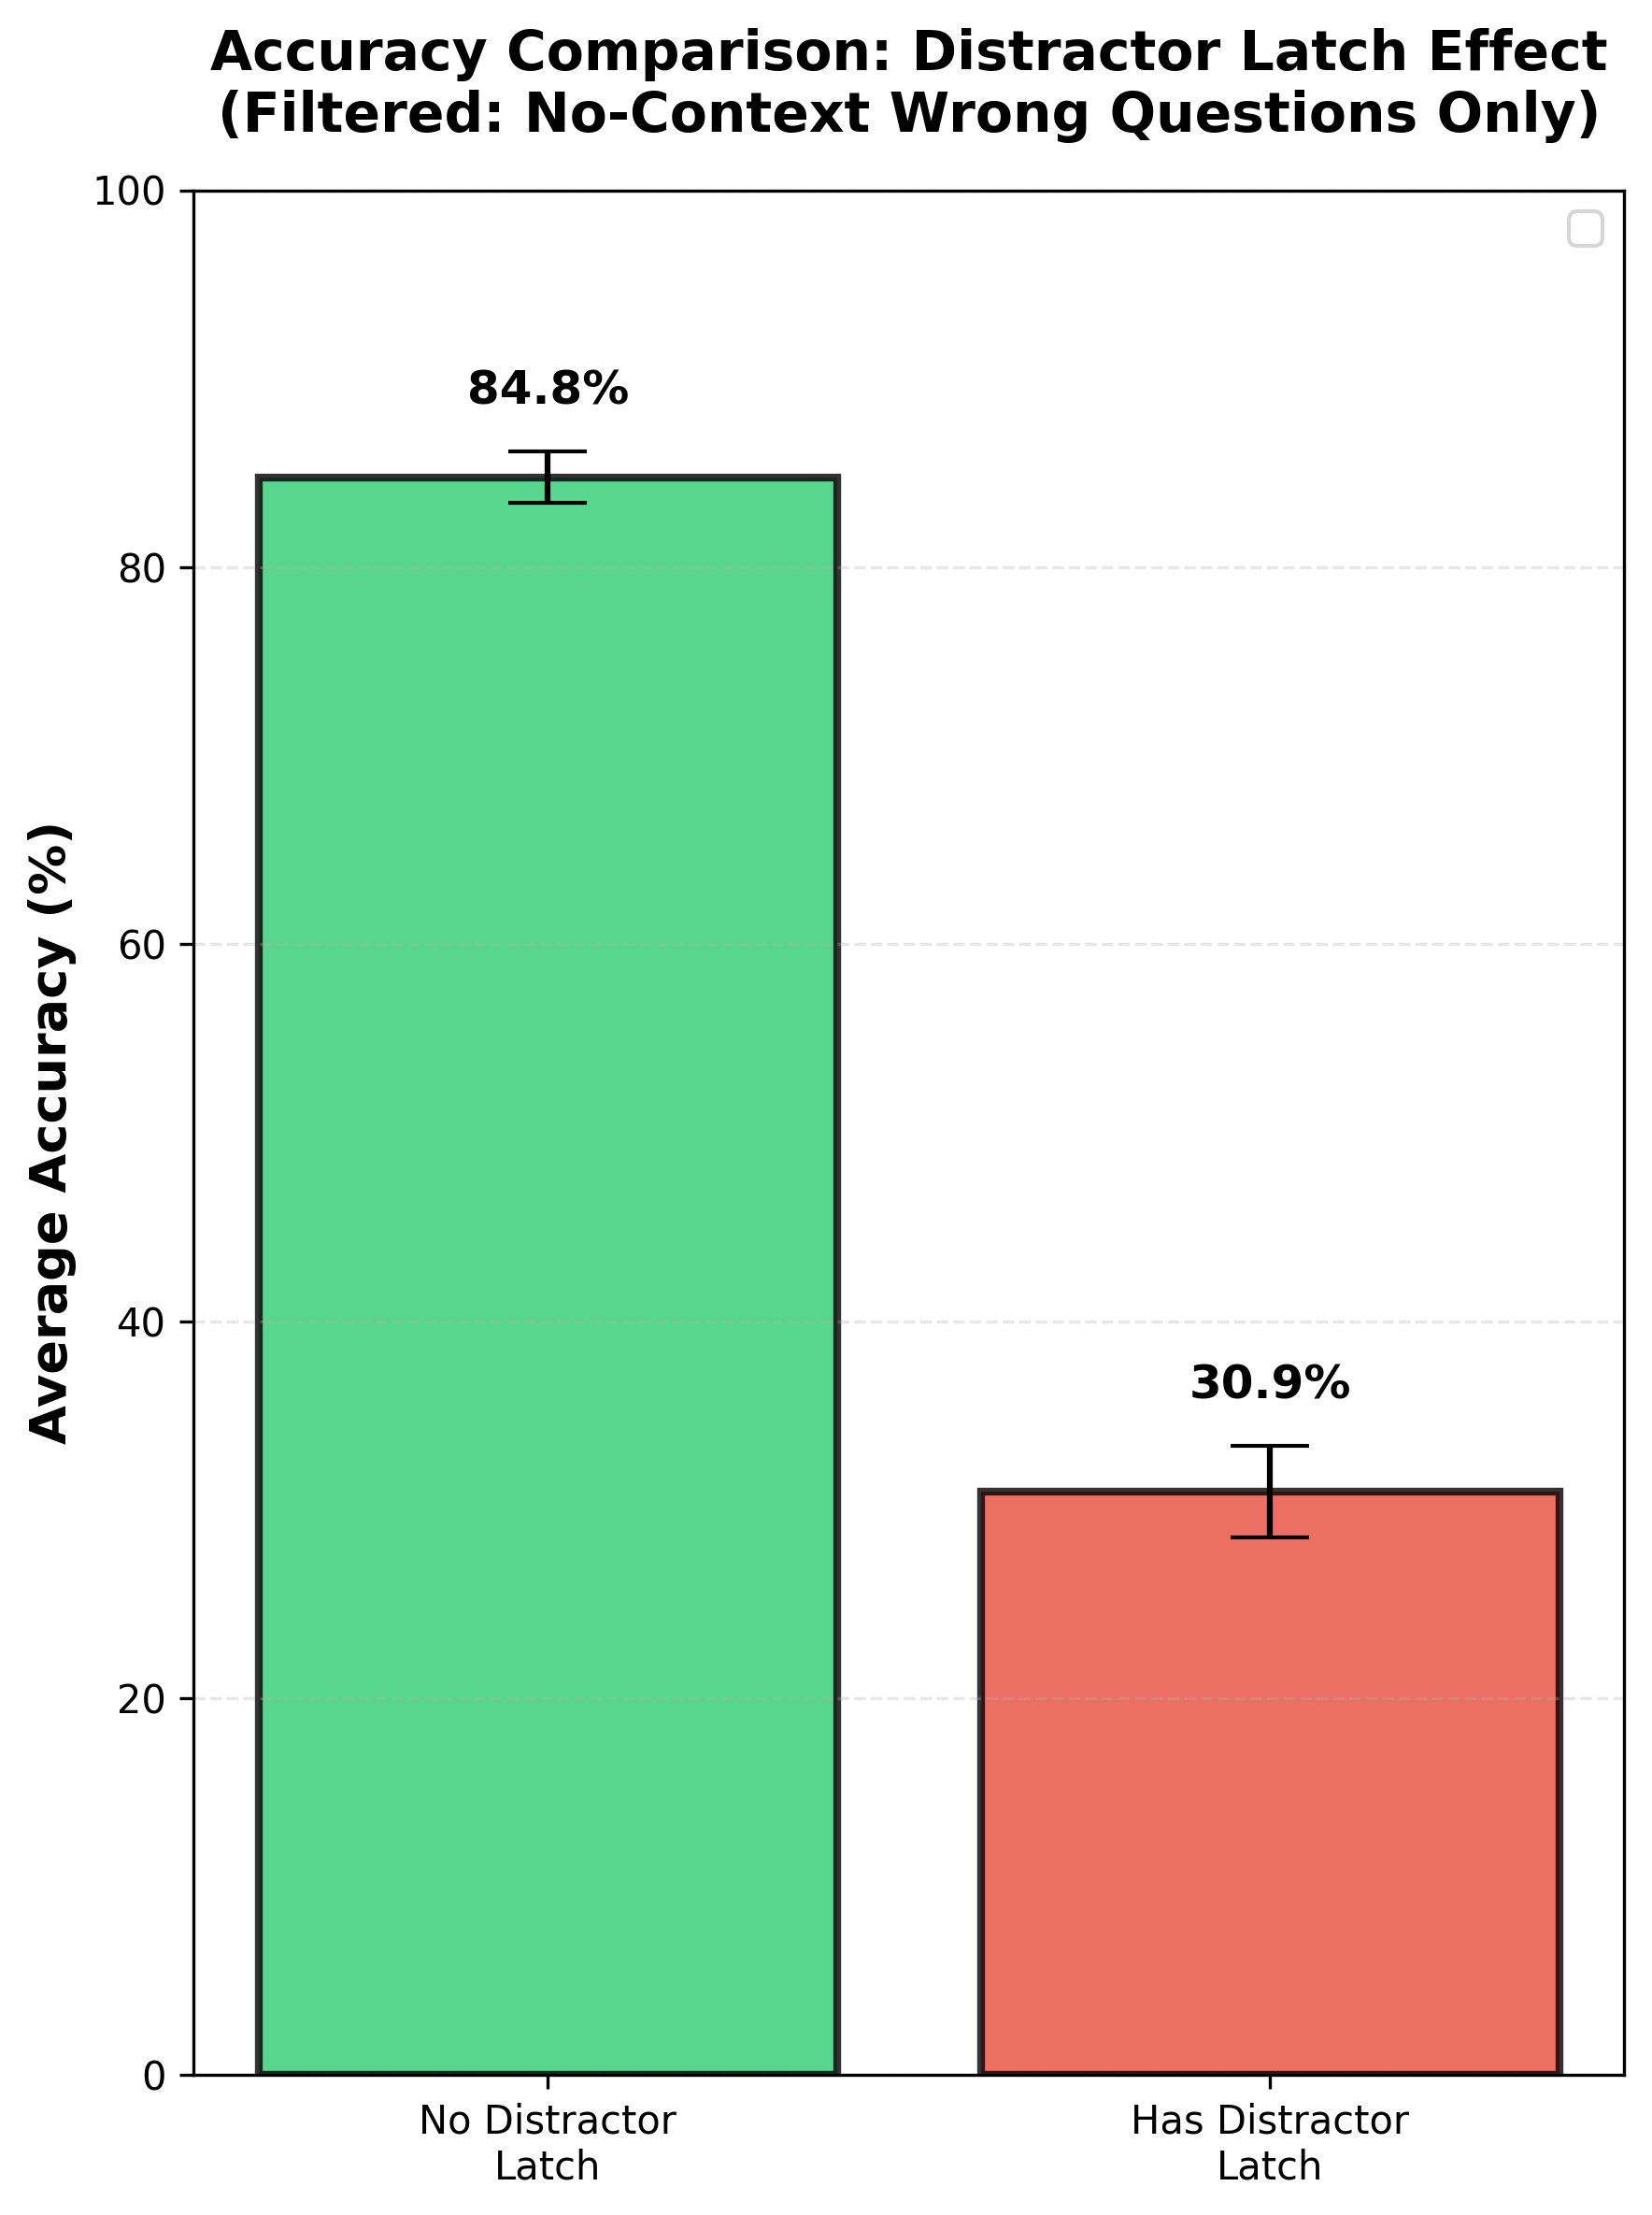
\includegraphics[width=\textwidth]{distractor_latch_accuracy_comparison.png}
%         \caption{Accuracy comparison}
%         \label{fig:distractor_accuracy_alt}
%     \end{subfigure}
%     \hfill
%     \begin{subfigure}[b]{0.32\textwidth}
%         \centering
%         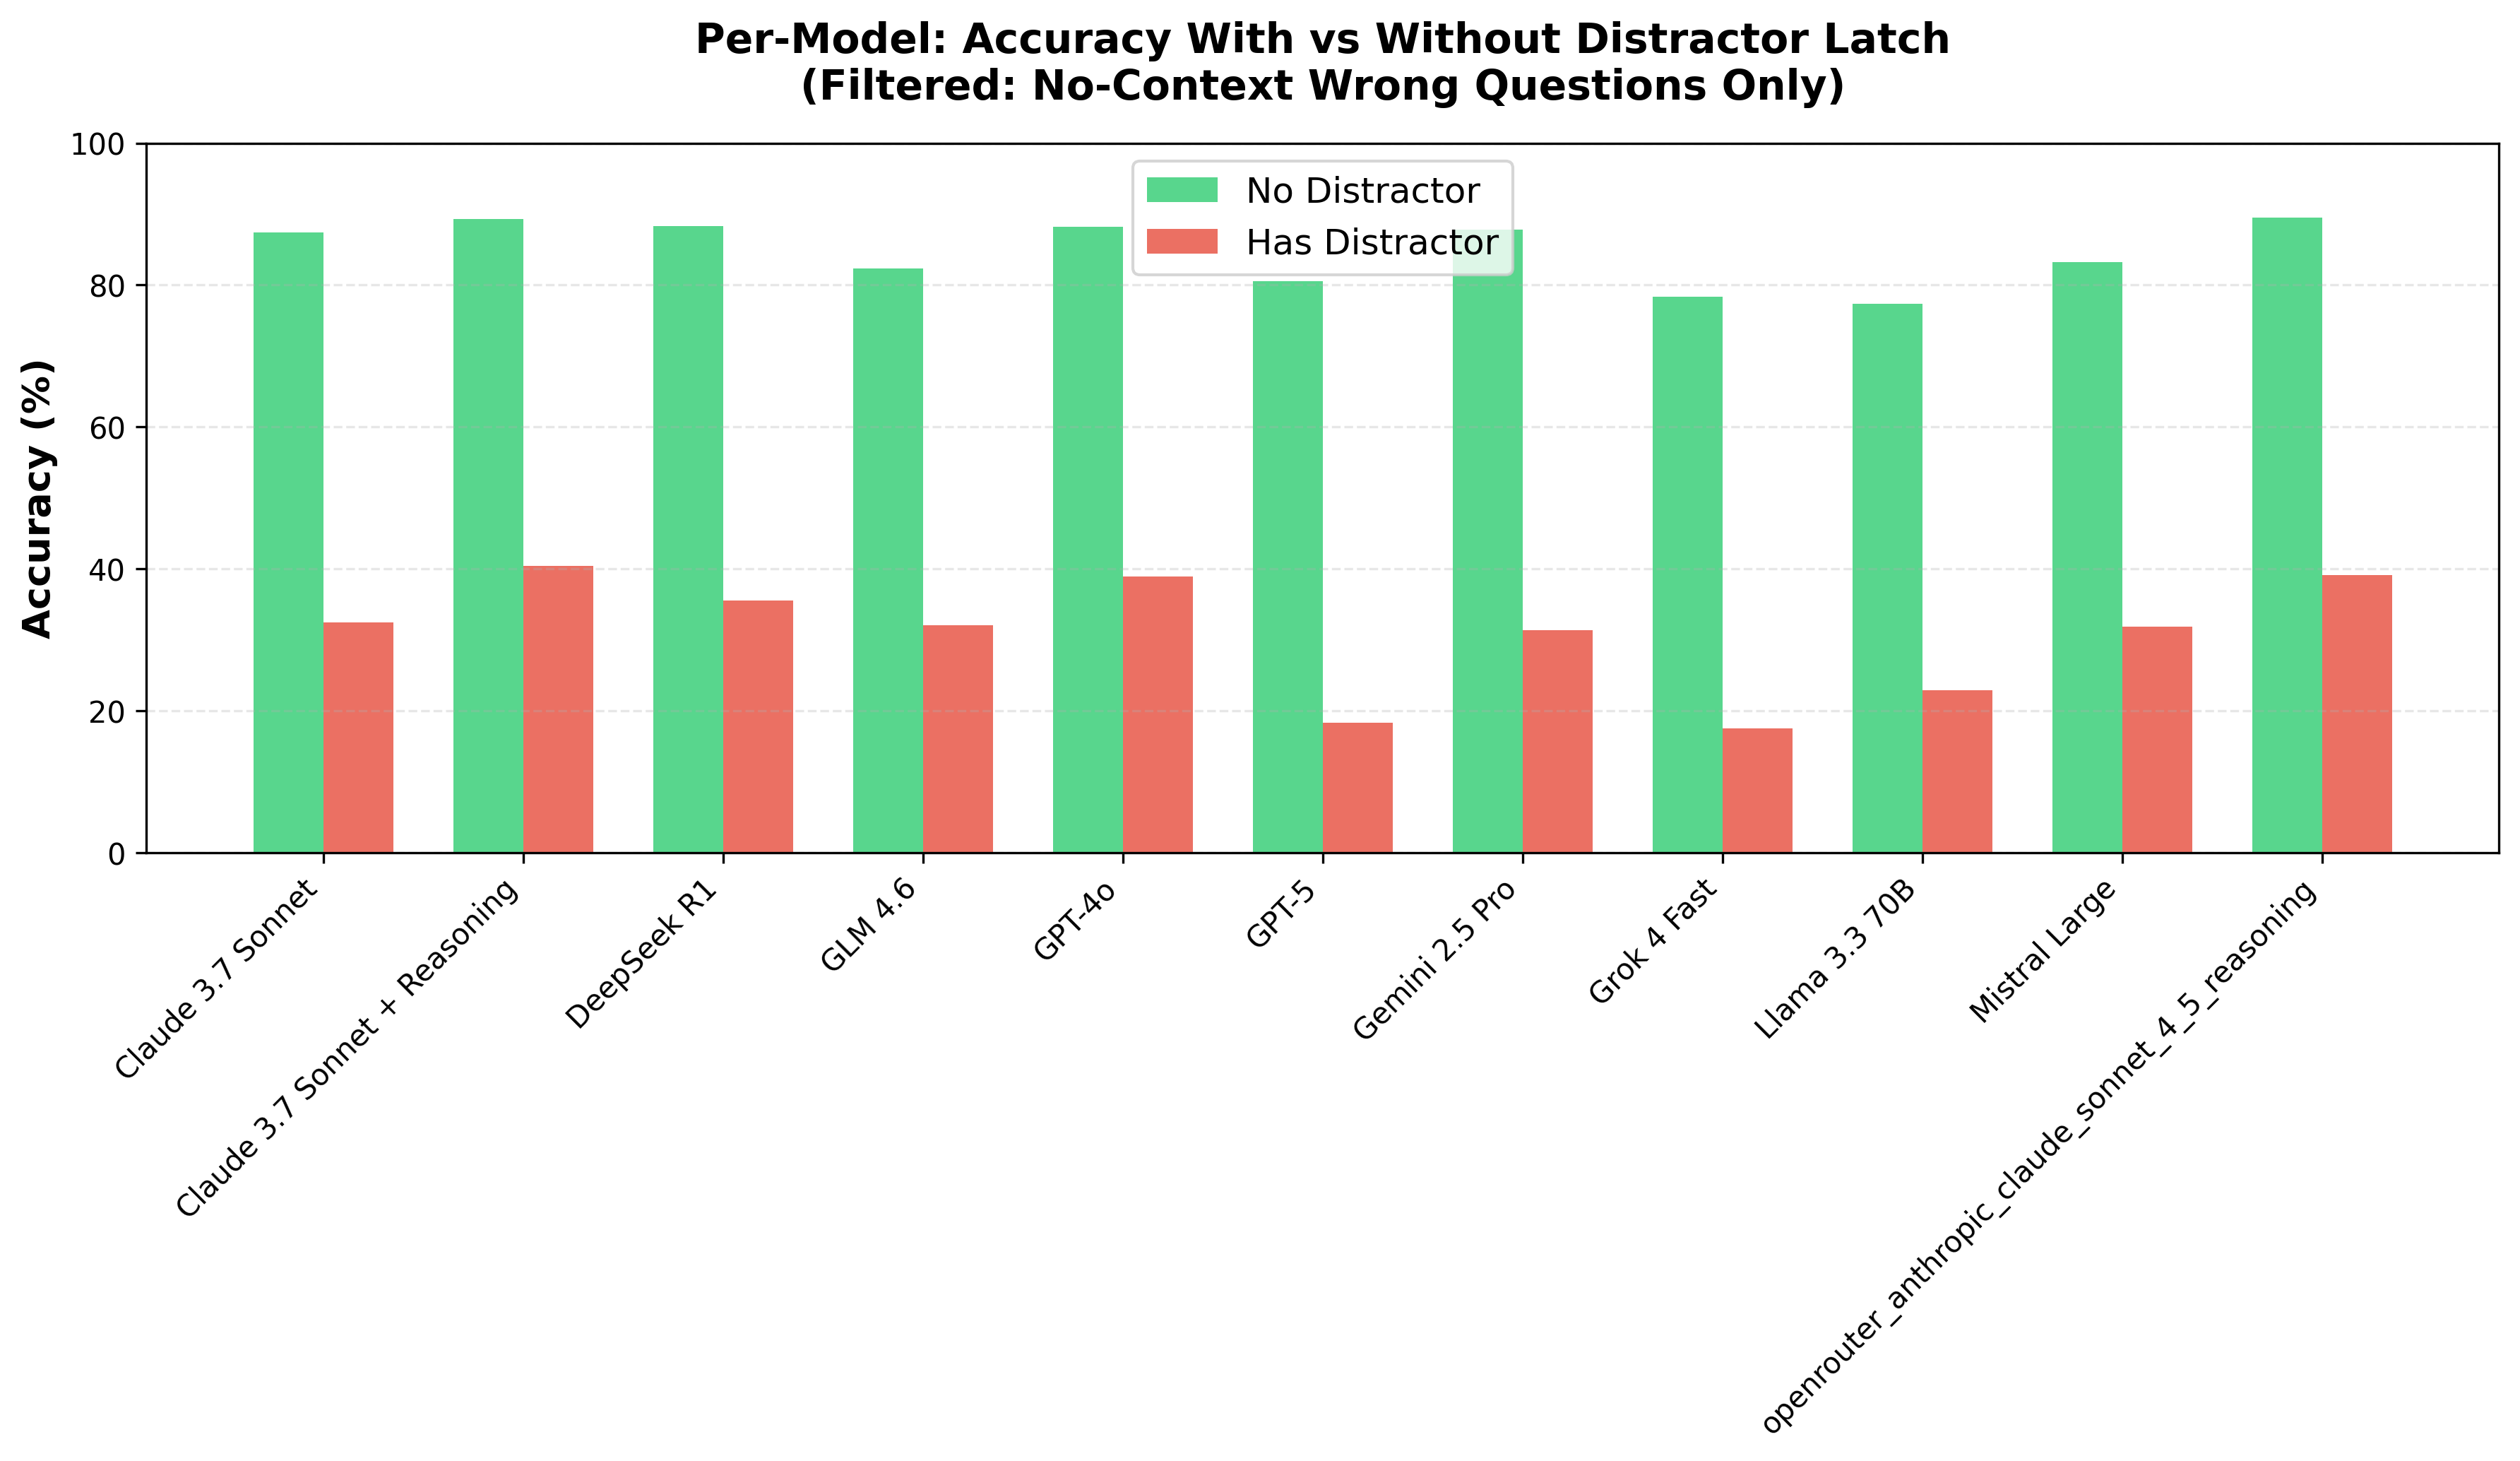
\includegraphics[width=\textwidth]{distractor_latch_per_model.png}
%         \caption{Per-model breakdown}
%         \label{fig:distractor_per_model_alt}
%     \end{subfigure}
%     \hfill
%     \begin{subfigure}[b]{0.32\textwidth}
%         \centering
%         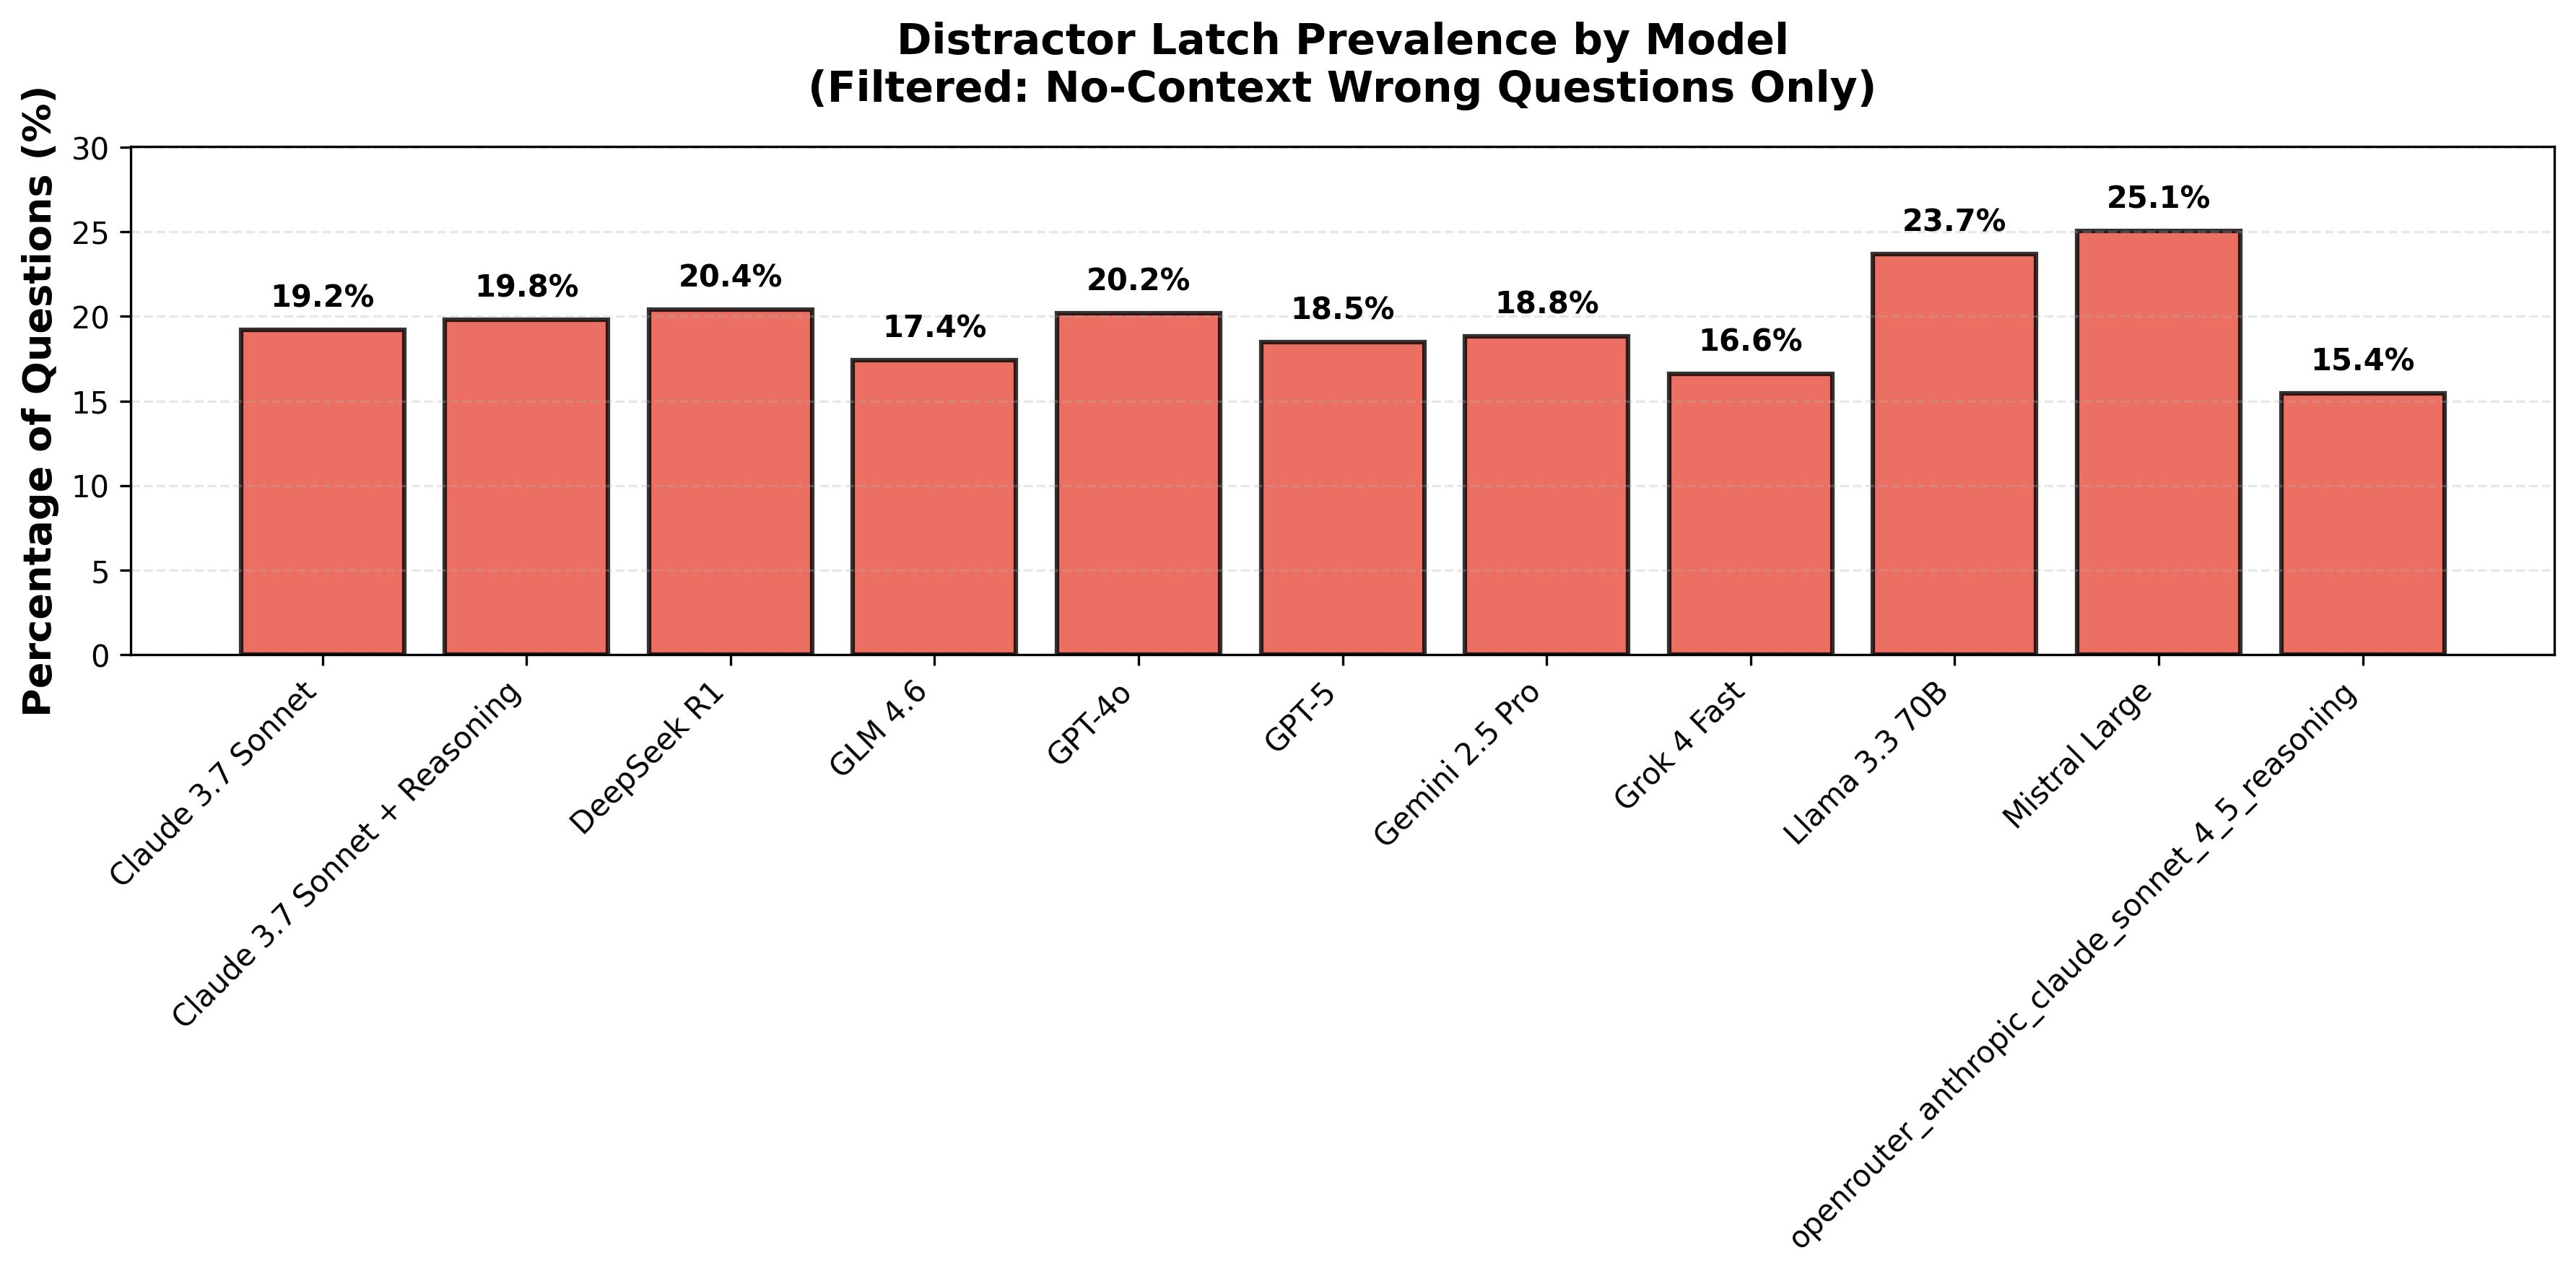
\includegraphics[width=\textwidth]{distractor_latch_prevalence.png}
%         \caption{Prevalence by model}
%         \label{fig:distractor_prevalence_alt}
%     \end{subfigure}
%     
%     \caption{Distractor latch analysis showing (a) overall impact, (b) per-model effects, and (c) prevalence rates.}
%     \label{fig:distractor_latch_analysis_alt}
% \end{figure}

% Note: Make sure to include the following in your LaTeX preamble:
% \usepackage{graphicx}
% \usepackage{subcaption}  % or \usepackage{subfig}
